\documentclass[bigger]{beamer}
\usepackage[utf8]{inputenc}
\usepackage[T1]{fontenc}
\usepackage{color}
\usepackage{graphicx}
\usepackage{eurosym}
\usepackage{parcolumns}

\DeclareGraphicsExtensions{.png,.pdf,.jpg}
\graphicspath{{./pics/}}

%Global Background must be put in preamble
\usebackgroundtemplate%
{%
    
\includegraphics[width=\paperwidth,height=\paperheight]{Design.jpg}%
}


\newcommand{\topic}[1]{{\huge{\textcolor{white}{\textbf{#1}}}}}
%\newcommand{\topic}[1]{\textbf{#1}}

\begin{document}
{
\usebackgroundtemplate{
\includegraphics[width=\paperwidth]{Back.jpg}}%
\begin{frame}
%Title: leer, vielleicht noch unsere Namen einfügen
\begin{figure}[H]
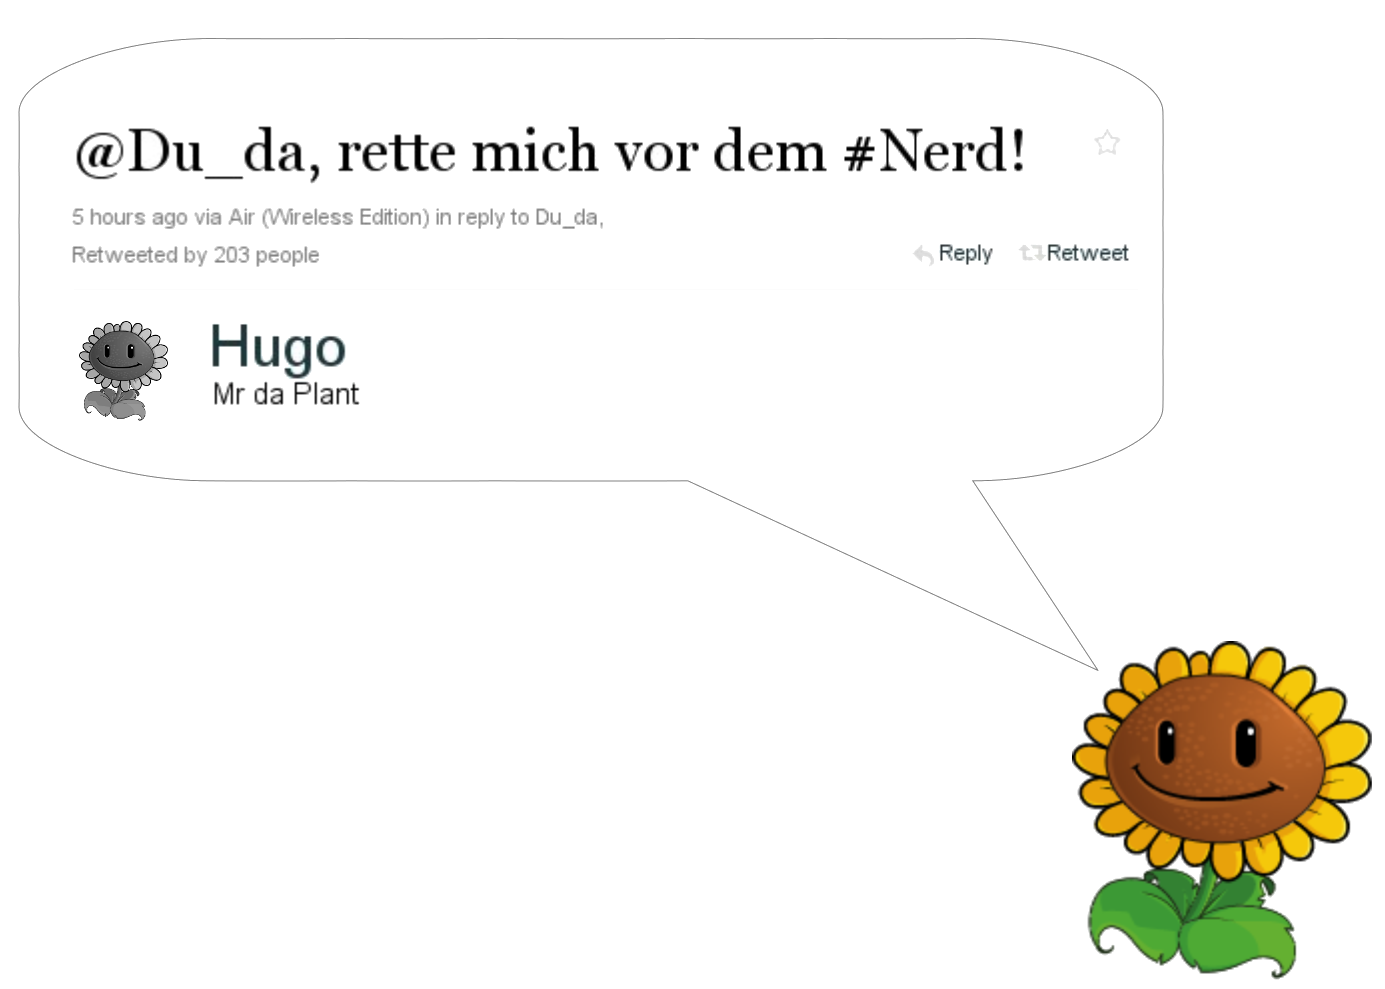
\includegraphics[width=350px]{SprechblaseOR.png}
\end{figure}

\end{frame}
}

\begin{frame}{\topic{Übersicht}}
   \begin{itemize}
      \item Auswahl existierender ähnlicher Projekte
      \item Vorstellung Plant Guard
      \item Zielgruppe
      \item Arbeitsstand
      \item Weitere Schritte
   \end{itemize}
\end{frame}

\begin{frame}{\topic{E-Plant}}
	\begin{itemize}
		\item Wird an die Pflanze angeklemmt
		\item Misst ähnlich wie ein EKG
		\item Umwelteinflüsse erkennen
		\item Wird noch nicht produziert
		\item \url{http://www.land-der-ideen.de/365-orte/preistraeger/e-plant-pflanzen-monitoring-sensor}
	\end{itemize}
\end{frame}

\begin{frame}{\topic{Botanicalls}}
	\begin{itemize}
		\item Twittert und/oder ruft an
		\item Nur Feuchtigkeit
		\item 100\$
		\item \url{http://www.botanicalls.com/}
	\end{itemize}
\end{frame}

\begin{frame}{\topic{Tomato Irrigation Project}}
	\begin{itemize}
		\item Twittert
		\item Feuchtigkeitssensor
		\item automatische Bewässerung mit Pumpe
		\item nicht mehr aktiv
		\item \url{http://picasaweb.google.com/joouni/WateringSystem}
		\item \url{https://twitter.com/tomaatit}
	\end{itemize}
\end{frame}

\begin{frame}{\topic{Giess-o-mat}}
	\begin{columns}[T]
		\begin{column}{.5\textwidth}
			\begin{itemize}
				\item automatisiertes Gießen
				\item Verwaltung der Pflanzen über Terminal
				\item Feuchtigkeitssensor
				\item \url{http://www.mikrocontroller.net/articles/Giess-o-mat}
			\end{itemize}
		\end{column}
		\begin{column}{.5\textwidth}
			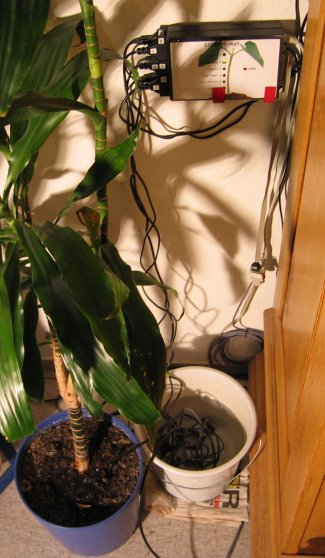
\includegraphics[width=0.55\linewidth]{Giessomat.jpg}
		\end{column}
	\end{columns}
\end{frame}

\begin{frame}{\topic{GardenBot}}
	\begin{itemize}
		\item Temperatur- und Feuchtigkeitsmessung
		\item automatisiertes Gießen
		\item Auch für den Garten gedacht
		\item (erstmal) nicht mehr aktiv
		\item \url{http://gardenbot.org/}
	\end{itemize}
\end{frame}

\begin{frame}{\topic{Koubachi}}
	\begin{itemize}
		\item Temperatur-, Feuchtigkeits- und Lichtsensor (nur mit Gerät)
		\item Wasser-, Düng-, Besprühplan auch ohne Gerät
		\item Gerät auch für mehrere Pflanzen, indoor und outdoor
		\item Config für Pflanzentypen im Internet
		\item Nur mit Iphone App oder Facebook-Account
		\item 90-200 Euro
		\item \url{http://www.koubachi.com/}
	\end{itemize}
\end{frame}

\begin{frame}{\topic{Parrot Flower Power}}
	\begin{itemize}
		\item Temperatur-, Feuchtigkeits- und Lichtsensor
		\item Düngerstandmessung
		\item Bluetooth + Smartphone
		\item Kommt irgendwann 2013 raus
		\item\url{http://www.parrot.com/flower-power/}
	\end{itemize}
\end{frame}

\begin{frame}{\topic{Plant irrigation system}}
	\begin{itemize}
		\item Reservoir wird am Blumentopf befestigt
		\item Wasser tropft in die Erde
	\end{itemize}
\end{frame}

\begin{frame}{\topic{Plant irrigation device}}
	\begin{itemize}
		\item Flasche steckt in der Erde
		\item Wasser tropft durch eine Kappe in die Erde
	\end{itemize}
\end{frame}
\begin{frame}{\topic{The "planned" guard}}
	\begin{itemize}
		\item Feuchtigkeitssensor
		\item Temperatursensor
		\item automatische Bewässerung
		\item Füllstandssensor
		\item Lichtsensor?
		\item einfache Möglichkeit zur Konfiguration
		\item ... und natürlich Tweets!
	\end{itemize}
\end{frame}

\begin{frame}{\topic{Abnehmer/Interessierte}}
	\begin{itemize}
		\item Neulinge, damit ihre erste Zimmerpflanze nicht ihre letzte wird
		\item Personen, die oft unterwegs sind und nicht jeden Tag zum gießen nach Hause kommen (können)
		\item Leute mit dem “braunen Daumen”, die trotzdem auf ein bisschen Grün nicht verzichten wollen
		\item Statistikhungrige (Wasserverbrauch, Lebenszeit, ...)
		\item Allen, die es einfach cool finden, wenn ihre Pflanze sich selber gießt
	\end{itemize}
\end{frame}

\begin{frame}{\topic{Bisherige Arbeiten}}
	\begin{itemize}
		\item Feuchtigkeitssensor für den Boden
		\item Temperatursensor
		\item Bewässerungsautomatisierung
		\item Grundgerüst der Software (https://github.com/jasinai/plant\_guard)
	\end{itemize}
\end{frame}
\begin{frame}
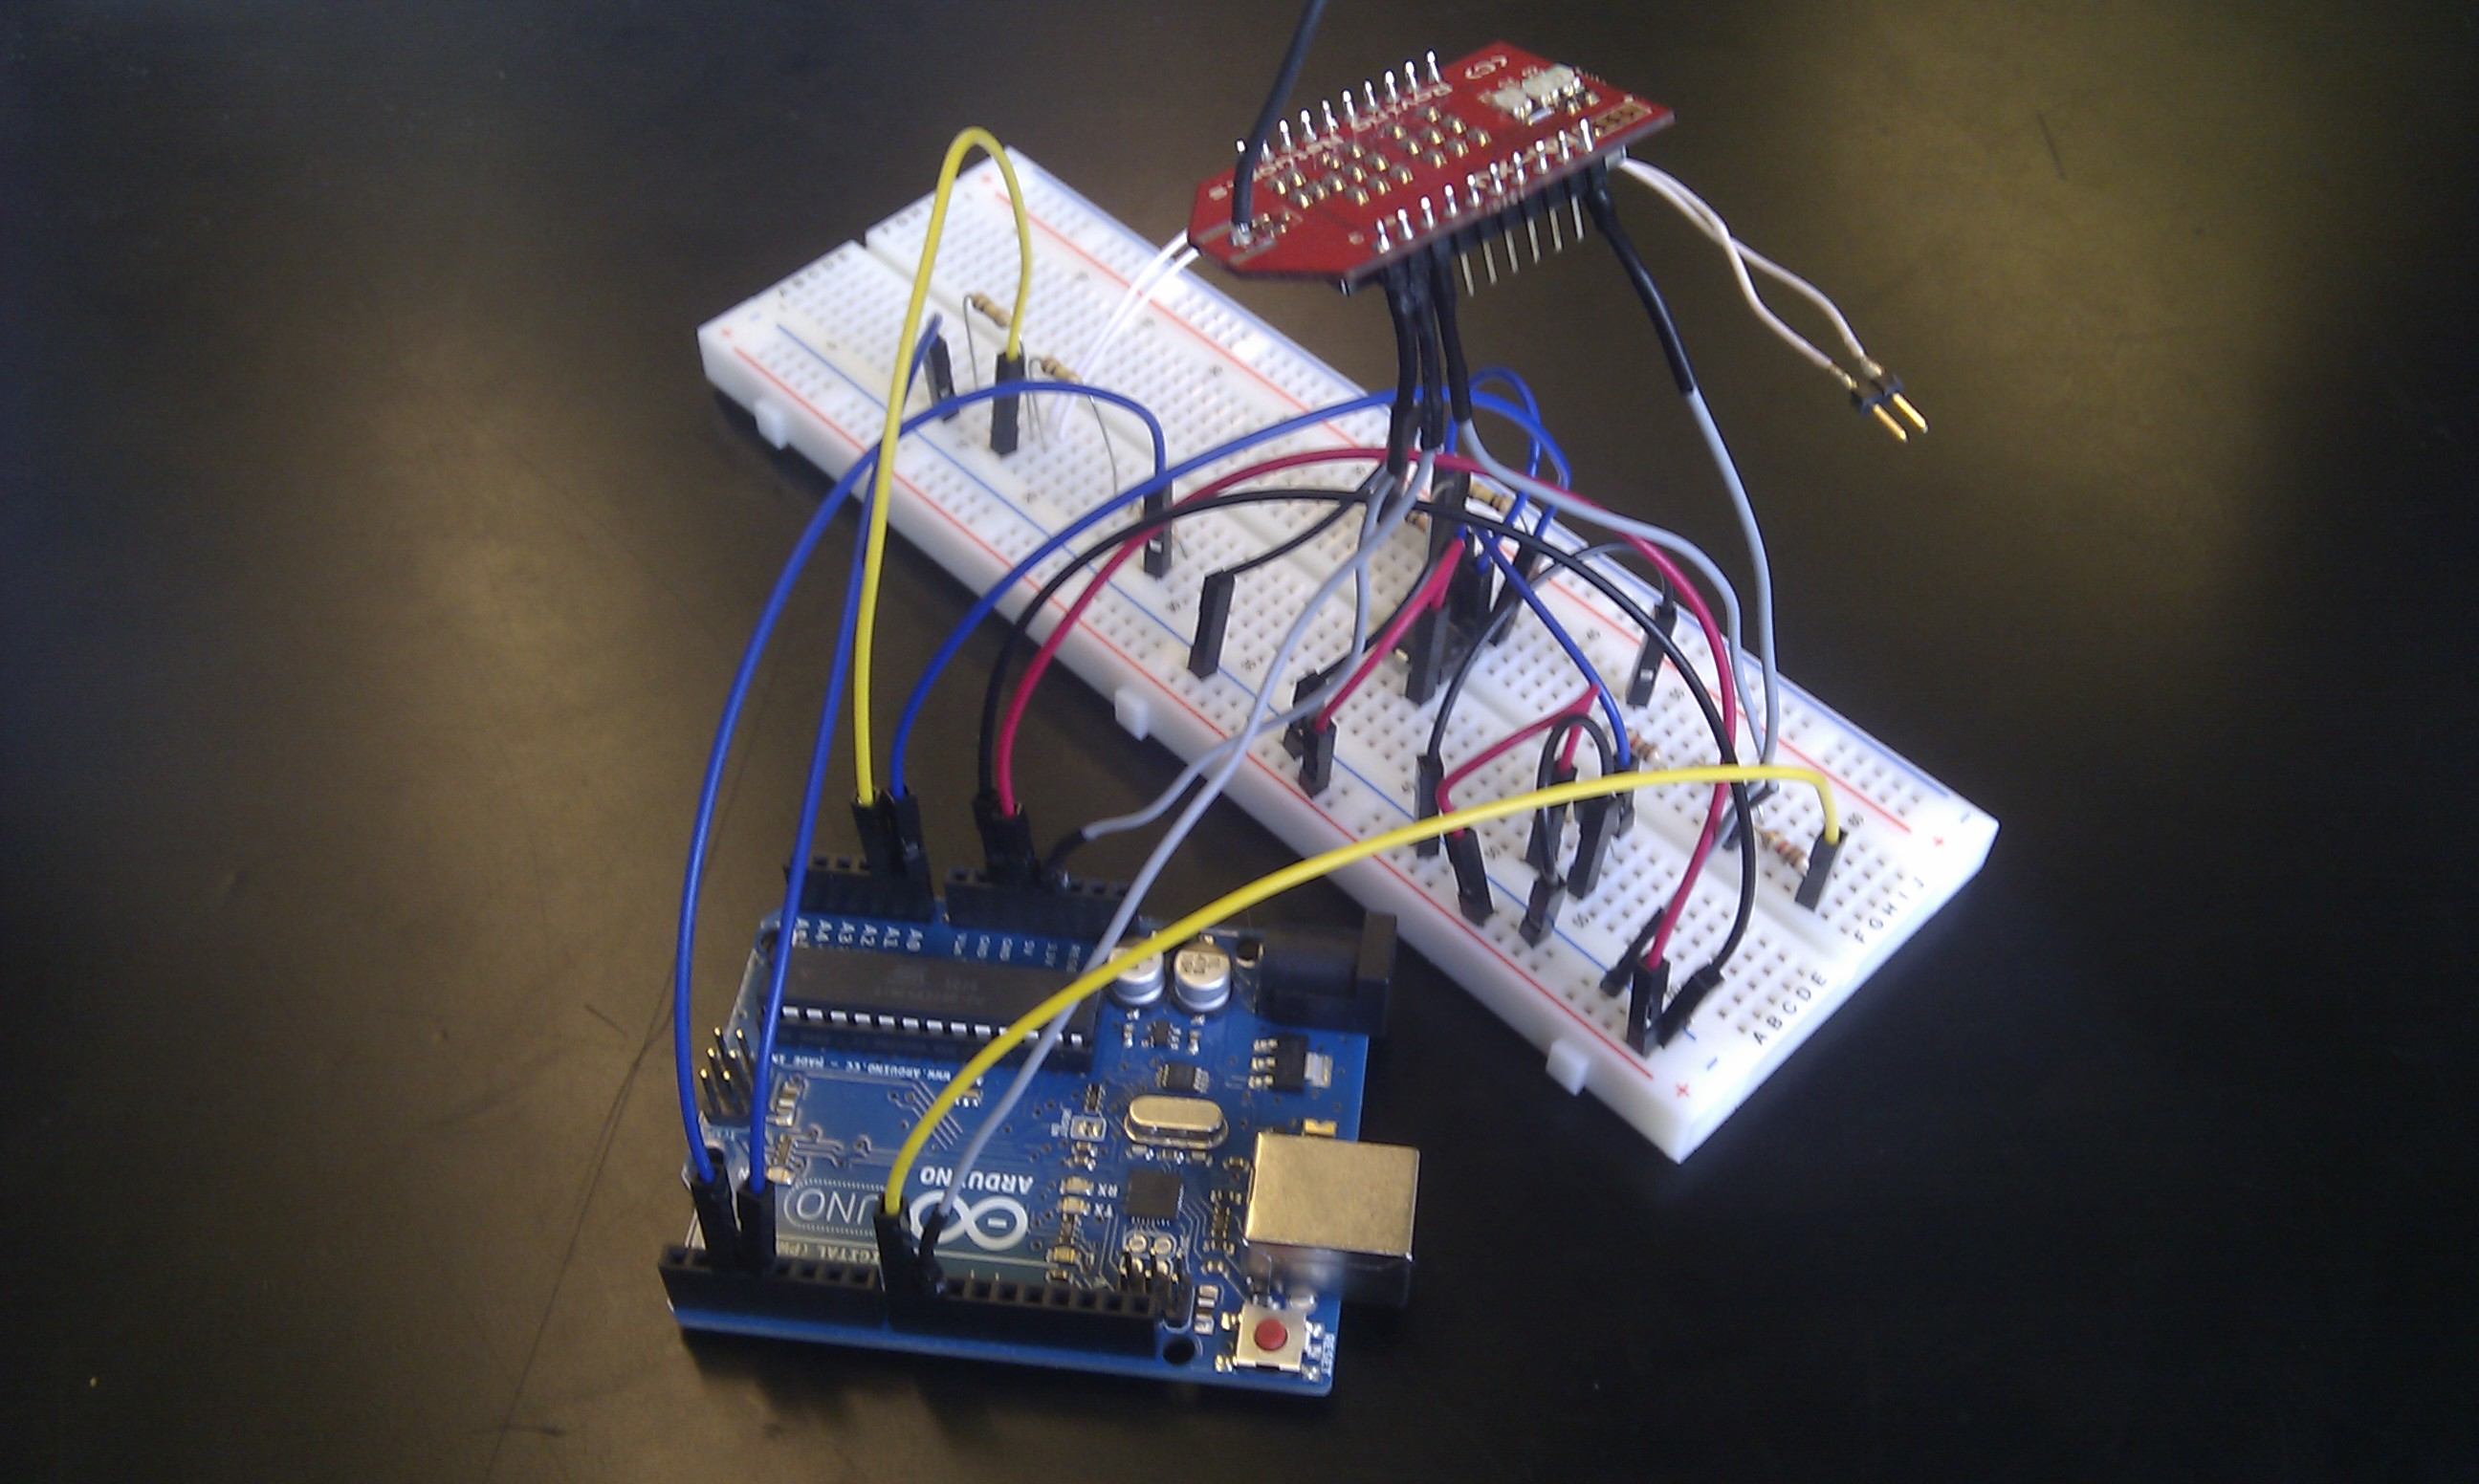
\includegraphics[width=350px]{board.jpg}
\end{frame}
\begin{frame}{\topic{Temperatursensor}}
	\begin{itemize}
		\item LM35 aus dem Starterkit
	\end{itemize}
\end{frame}

\begin{frame}{\topic{Feuchtigkeitssensor}}
		\begin{itemize}
			\item Stiftleisten oder Nägel in Gips
			\item Korrisionsschutz: Wechselstrom
		\end{itemize}
		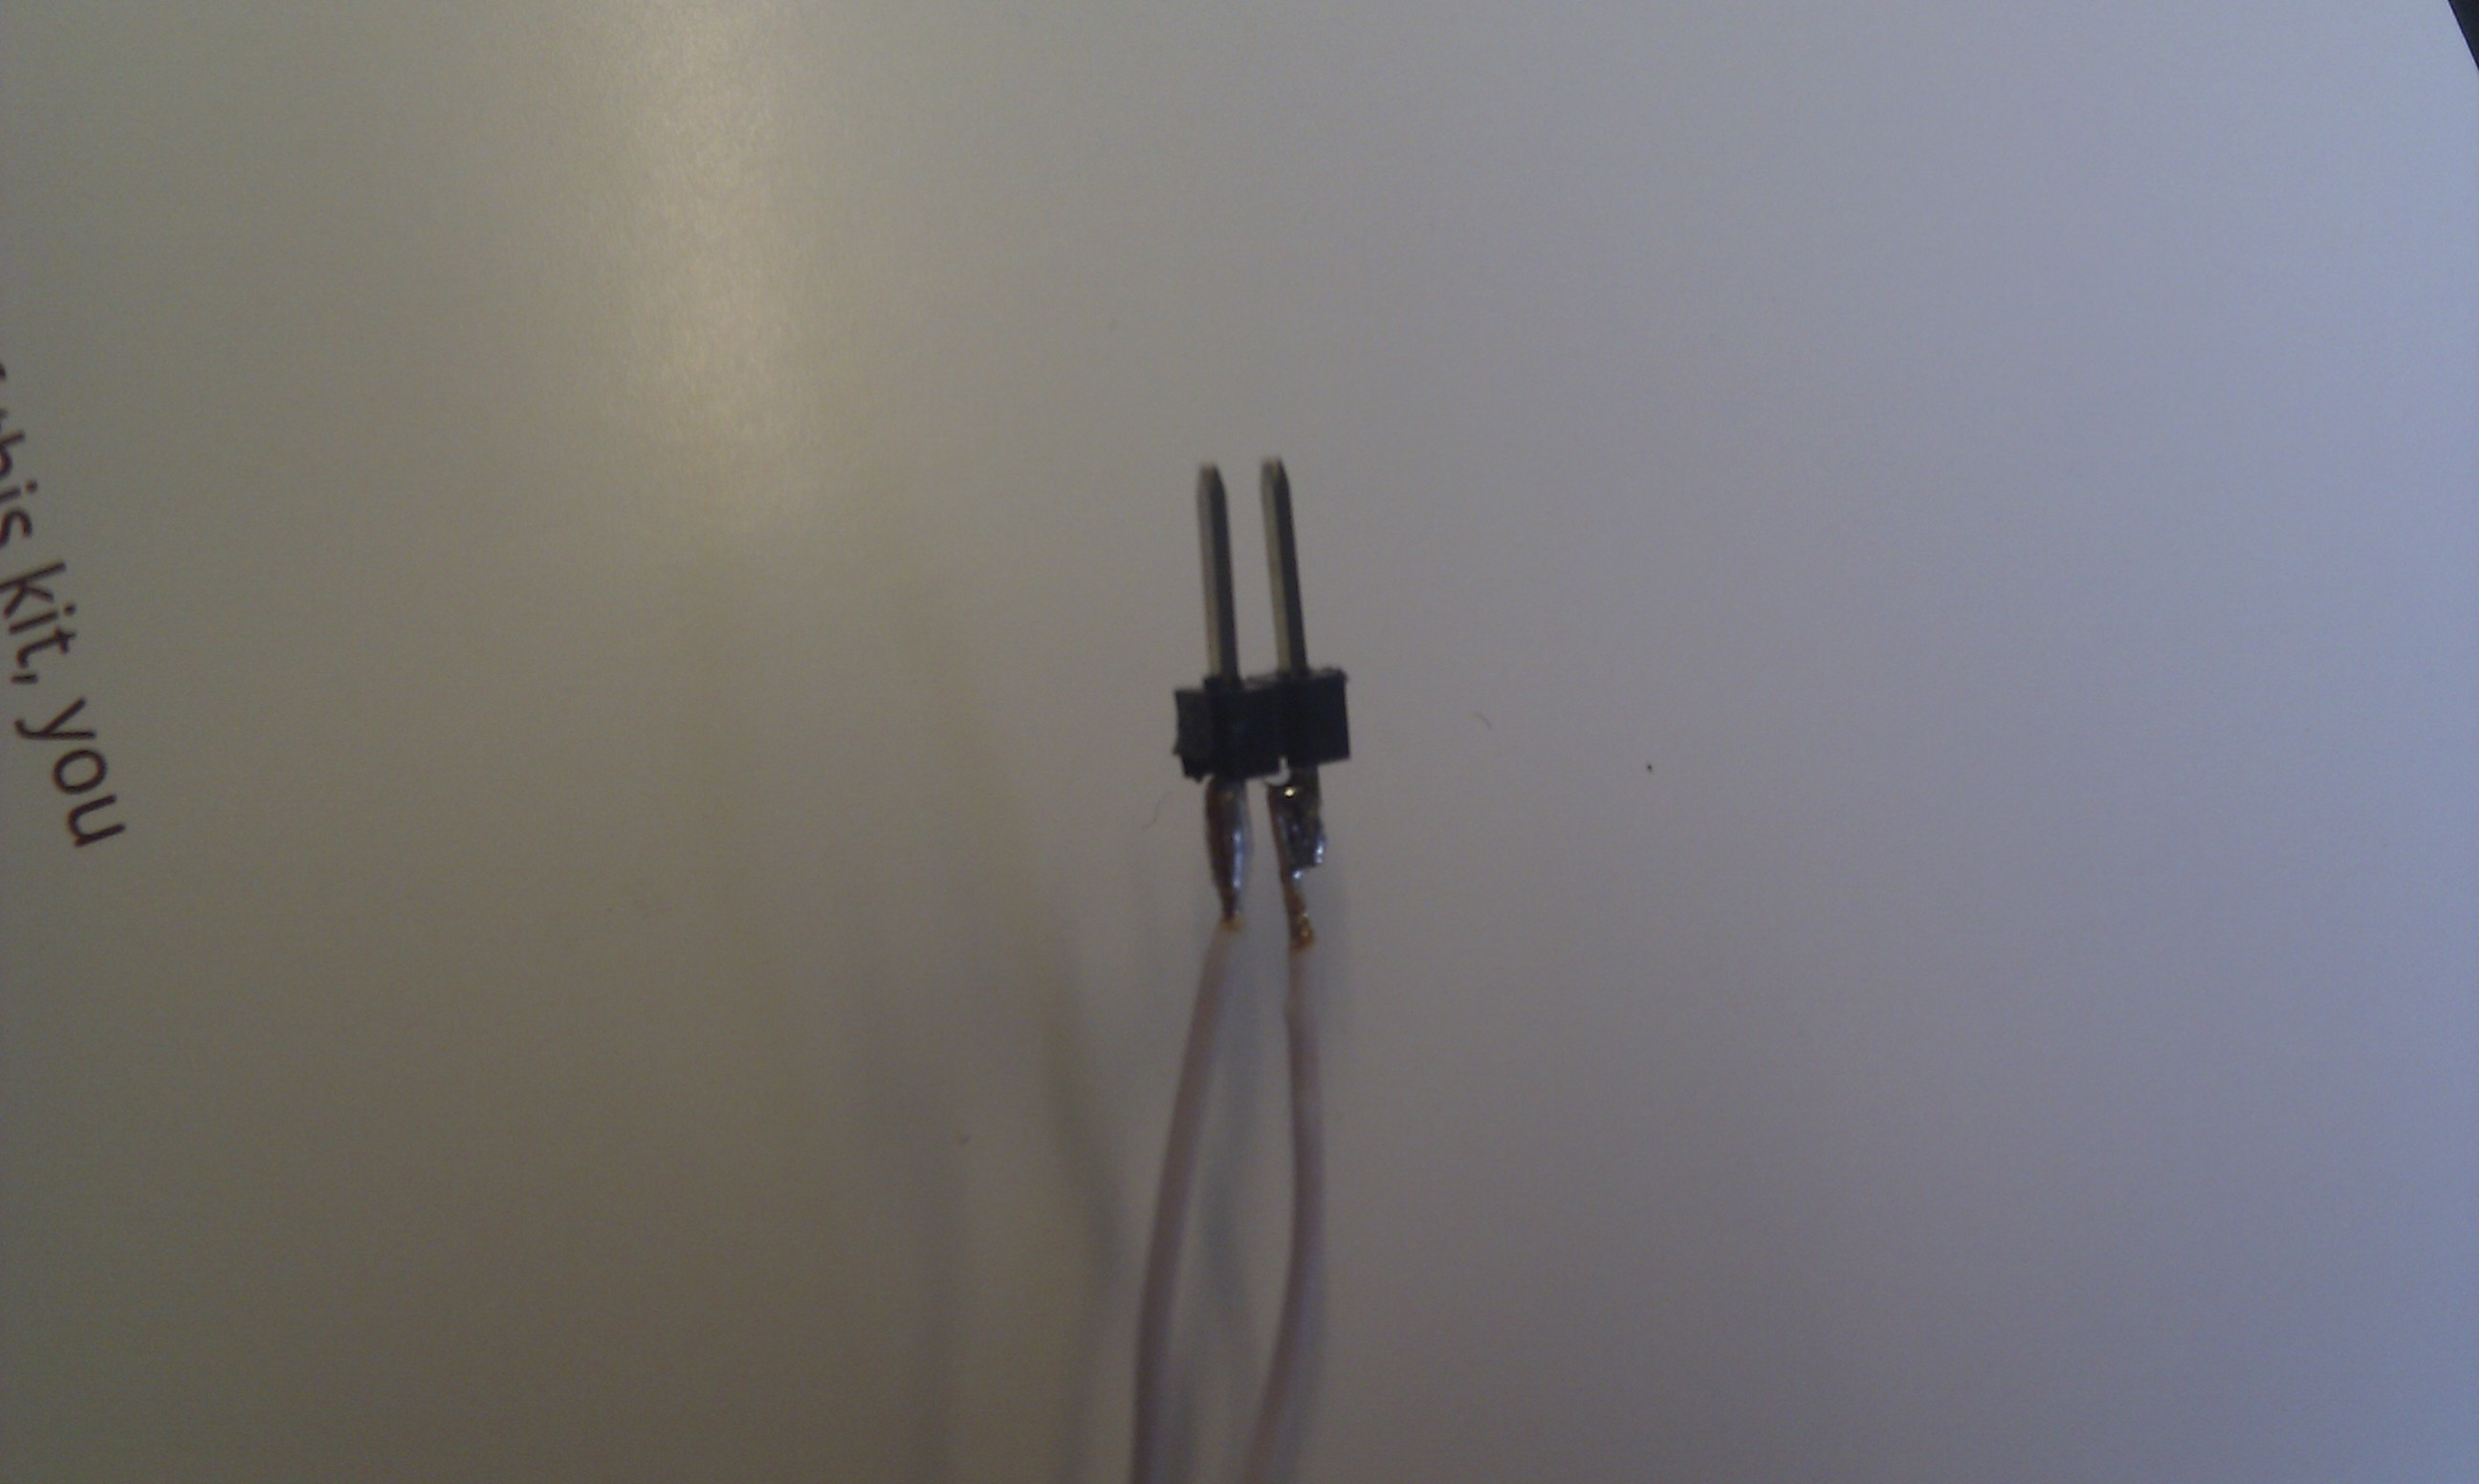
\includegraphics[width=350px]{IMAG0560.jpg}
\end{frame}

\begin{frame}{\topic{Bewässerung}}
       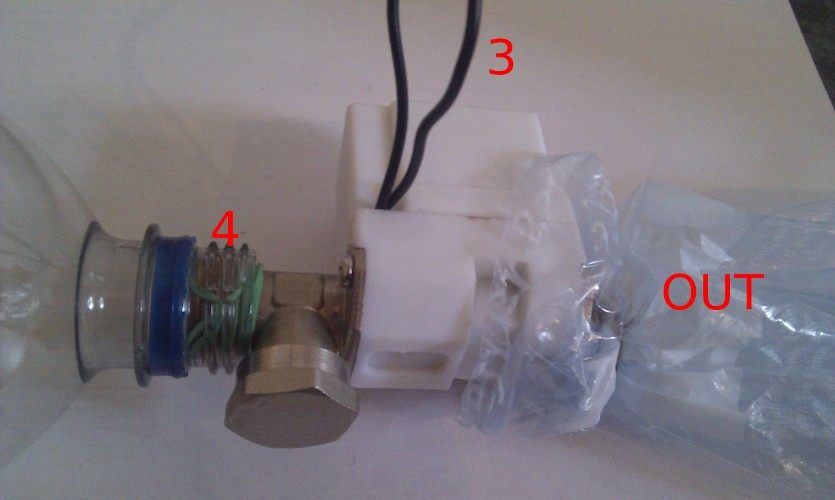
\includegraphics[width=350px]{Anschluss.jpg}
\end{frame}

\begin{frame}{\topic{Bewässerung}}
    \begin{columns}
      \column[c]{.50\textwidth}
        \begin{enumerate}
			\item verbreiterte Stellfläche
			\item Messkabel
			\item Ventilansteuerung
			\item Verbindung Vorrat $\rightarrow$ Ventil
        \end{enumerate}
      \column[c]{.50\textwidth}
        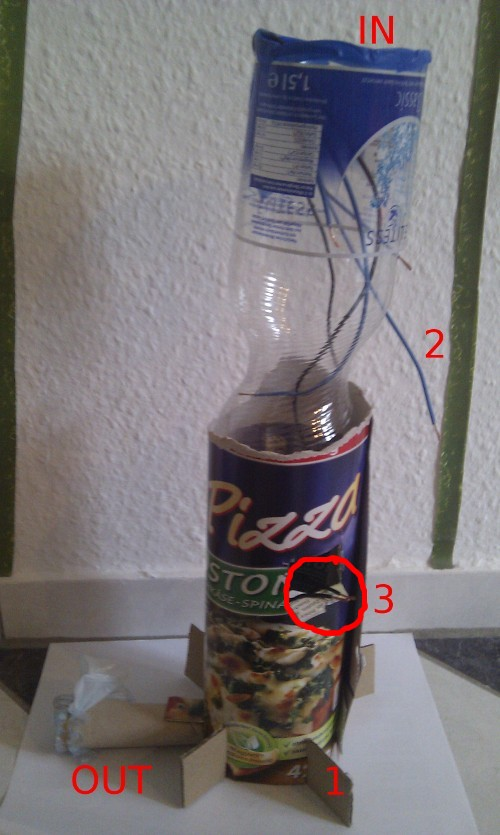
\includegraphics[width=150px]{System.jpg}
    \end{columns}
\end{frame} 

\begin{frame}{\topic{Bewässerung}}
	\begin{itemize}
		\item Die Ventile schalten sehr leise
		\item Es wird Lageenergie genutzt
		\item mit Ventil, Pfand, Platinen, Schlauch, Dichtung, Kabeln ca. 10\euro
		\newline
		\item Pappkonstruktion ist \textbf{sehr} wasserempfindlich!
		\item Eine Konstruktion je Pflanze nötig
	\end{itemize}
\end{frame} 


\begin{frame}{\topic{Arduino}}
	\begin{itemize}
		\item mit Direktanschluss können 2 Pflanzen überwacht werden
		\item verschiedene Upgrades möglich (Anzahl++, Verteilung der Pflanzen, ...)
		\item Verpackung zum Schutz vor Wasserschäden
		\item Twittert schon
		\newline
		\item Jetzt noch messen, verarbeiten und ausgeben in einem Programm zusammenbringen
	\end{itemize}
\end{frame}

\begin{frame}{\topic{Tweets}}
	\begin{itemize}
		\item "Ich sitze schon x Tage im Dunkeln! Hat da wer die Rollos vergessen?"
		\item "Einen wunderschönen Morgen…" / "Gute Nacht!" (Uhr/Lichtsensor)
		\item "Mir ist langweilig... komm doch mal vorbei und erzähl mir was!” (Zufallsereignis)
		\item "Wasserstand niedrig: Raum x: Pflanzen-ID, Raum y: Hugo, Otto"
		\item "Die Pflanzen Hugo, Otto und Karla wurden erfolgreich gewässert!"
	\end{itemize}
\end{frame}


\begin{frame}{\topic{Vorteile}}
	\begin{itemize}
		\item Arbeitsteilung wird sehr einfach (nicht zu oft/wenig gegossen)
		\item Urlaubsvertretung braucht nur Zugriff auf Twitterdaten
		\item Gießen auf Vorrat möglich
		\item Im Gegensatz zur Konkurrenz könnten wir unser Projekt frei erweitern
		\item ... und kriegen die Daten "weltweit"!
	\end{itemize}
\end{frame}


\begin{frame}{\topic{Nachteile}}
	\begin{itemize}
		\item Stromausfall $\Rightarrow$ es wird nicht gegossen!
		\item Behälter könnte umkippen oder die Dichtung versagen
		\item Pflanzenbesitzer könnte seltener nach Schädlingen usw suchen, da "alles" automatisch funktioniert
		\item (der Behälter muss mindestens auf Höhe der Pflanze sein)
	\end{itemize}
\end{frame}


\begin{frame}{\topic{Weiteres Vorhaben}}
	\begin{itemize}
		\item Basis-Version lauffähig machen
		\item Konfiguration ermöglichen (z.B. Webinterface)
		\item Gießsystem abdichten und klonen
		\item ein Opfer für die Beta finden
	\end{itemize}
	\begin{flushright}
		
\includegraphics[width=100px]{bloody2.png}
	\end{flushright}

\end{frame}


\begin{frame}{\topic{mögliche, nicht eingeplante Ideen}}
	\begin{itemize}
		\item mehr Sensoren (z.B. Fenster offen, Barometer, ...)
		\item mehr Pflanzen (mehr Anschlüsse durch Multiplexing / Bus / Wireless-Verbindung)
		\item "freie" Erweiterung durch User
	\end{itemize}
\end{frame}


{
\usebackgroundtemplate{
\includegraphics[width=\paperwidth]{Back.jpg}}%
\begin{frame}{}
	\begin{figure}[H]
		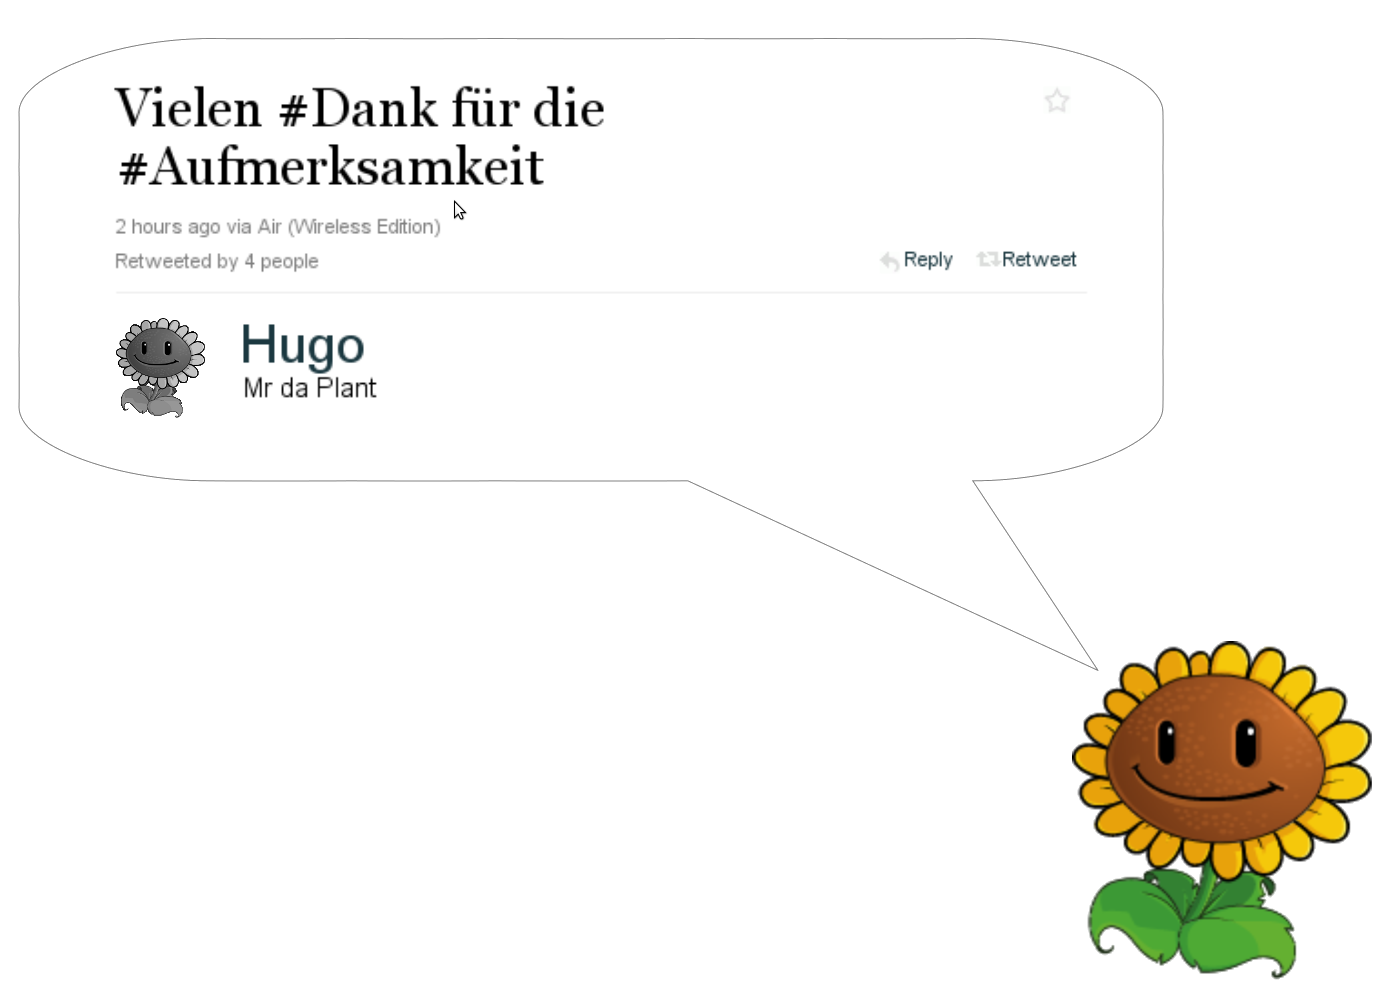
\includegraphics[width=350px]{Danke.png}
	\end{figure}
\end{frame}
}


\end{document}
